\documentclass[11pt,a4paper]{article}
\usepackage{fontspec}
\setmainfont{TeX Gyre Pagella}
\newfontfamily\headfont{Inter}[UprightFont=*-ExtraBold,BoldFont=*-ExtraBold,Extension=.otf,Path=/usr/share/fonts/opentype/inter/]
\usepackage[a4paper,margin=2.3cm]{geometry}
\usepackage{graphicx,booktabs,float,caption,array,xcolor,longtable}
\usepackage{xurl}
\usepackage[hidelinks]{hyperref}
\usepackage{titlesec}
\usepackage[round]{natbib}
\usepackage{setspace}
\setstretch{1.05}
\renewcommand{\topfraction}{0.9}
\renewcommand{\bottomfraction}{0.8}
\renewcommand{\textfraction}{0.1}
\renewcommand{\floatpagefraction}{0.75}
\setlength{\parindent}{0pt}
\setlength{\parskip}{0.55em}
\titleformat{\section}{\headfont\Large}{\thesection}{0.8em}{}
\titleformat{\subsection}{\headfont\large}{\thesubsection}{0.8em}{}
\captionsetup{font=small,labelfont=bf}
\urlstyle{same}
\hypersetup{pdftitle={Britain's Sunless Valleys},pdfauthor={Tristan Hotham}}

\begin{document}
\begin{center}
{\Large\bfseries Britain's Sunless Valleys\par}
\vspace{0.4em}
{\large Where terrain hides the winter sun, computed for every UK settlement and every 175 m of Britain and Ireland\par}
\vspace{1.2em}
{\large Tristan Hotham\par}
\vspace{0.3em}
{\small Independent researcher\\
ORCID: 0000-0003-4931-9349\\
DOI: https://doi.org/10.5281/zenodo.24055580\par}
\vspace{0.8em}
2026
\end{center}

\begin{quote}
\small
\begin{center}\textbf{Abstract}\end{center}
Around the winter solstice the noon sun stands between 6.6 and 16.6 degrees above the horizon in Britain, low enough for hills to hide it. I compute the terrain horizon from the open AWS Terrain Tiles (zoom 10, about 90 m) for 36,692 living settlements in the United Kingdom recorded in Wikidata and for 9,716,368 land squares of about 175 m covering Britain and Ireland, and combine it with the sun's path to give the minutes of direct sun on 21 December and the number of days around the solstice with none. Against a flat horizon the median settlement loses 18 minutes of solstice sunshine; 14\% lose at least an hour and 64 get no direct sun at all, 41 of them in Scotland and 15 in Wales. The longest runs without direct sun are in the western Highlands, led by Camas-luinie (123 days); Kinlochleven, a village of 810, goes 109 days. The count of 64 keeps a settlement only if it is also sunless at the OpenStreetMap point for the same place where one exists: 84 Wikidata points get no direct sun, but 20 of them get some at their OpenStreetMap point. 4,956 km$^2$ of UK land and 464 km$^2$ of Ireland get no direct sun on the solstice. The results describe terrain shadow only, at the resolution of the terrain model, with no buildings, trees or cloud.

\textbf{Keywords:} winter solstice; terrain horizon; topographic shading; insolation; digital elevation model; settlements; Scotland; Wales; Lake District
\end{quote}

\section{Introduction}
In the deep valleys of the Alps and Norway, places that lose the sun for weeks each winter are well known. Bristen, in the Maderanertal in the Swiss canton of Uri, is said to go about four months without it \citep{bluewin}; Rjukan in Norway, without direct sun from late September to March, has lit its town square since 2013 with mirrors on the mountainside above \citep{opn2013} and has celebrated the sun's return each spring with a festival since 1925 \citep{rjukan}. Britain's mountains are lower, but its latitude is higher: on 21 December the noon sun reaches 16.6 degrees at 50\textdegree{}N and only 6.6 degrees at 60\textdegree{}N, and for most of the short day it is lower still and far round to the south east or south west. A slope of a few hundred metres within a couple of kilometres to the south is enough to hide it. This paper asks which places in Britain get no direct sunshine for days or weeks around the winter solstice because terrain blocks the low sun, and how much of the shortest day's sunshine hills take from everywhere else.

Horizon angles from digital elevation models are a standard ingredient of solar radiation models \citep{dozier1981,hofierka2002}. Here they are applied at national scale to a gazetteer of settlements, so that every town and village in the United Kingdom gets a skyline and a count of sunless days, and to a regular grid, so that the pattern can be mapped.

\section{Data}
\textbf{Terrain.} The AWS Terrain Tiles (Mapzen's Terrarium encoding) at zoom 10 cover the area from 10.8\textdegree{}W to 2.0\textdegree{}E and 49.8\textdegree{}N to 61.0\textdegree{}N in 2,146 tiles of 256 by 256 cells, about 88 m across at 55\textdegree{}N. Over land in Britain and Ireland the heights come chiefly from the Shuttle Radar Topography Mission \citep{farr2007}. The tiles carry a few spikes and pits; I replaced any cell standing more than 150 m off the median of its 7 by 7 neighbourhood, or more than 60 m above the highest (below the lowest) of its eight neighbours, by that median, repeating until none remained (993 cells). Land is the Natural Earth outline of the United Kingdom, Ireland and the Isle of Man where the terrain is above $-8$ m.

\textbf{Settlements.} Wikidata \citep{wikidata} lists 69,384 rows of UK settlements with coordinates and types. I kept one point per item and only living settlements (types such as village, hamlet, town, suburb, locality or human settlement, and not hill forts, deserted or former villages, religious houses, camps or ski areas), leaving 36,692 places in the grid, 13,767 of them with a population. Each was assigned a county and nation from the ONS boundaries.

\section{Method}
\textbf{Horizon.} From each point, 2 m above the interpolated ground, I traced rays every degree of azimuth from 60\textdegree{} to 300\textdegree{} (east north east through south to west north west) out to 30 km. Samples start 80 m out and step by 80 m or 4\% of the distance, whichever is larger. At each sample the elevation angle of the bilinearly interpolated terrain is
\[ \tan\theta = \frac{h - h_0 - d^2 / (2R/(1-k))}{d}, \]
with $R$ the Earth's radius and $k = 0.13$ the standard coefficient of terrestrial refraction, and the horizon is the largest angle along the ray. For the grid I did the same from the centre of each 2 by 2 block of terrain cells (about 175 m), every 2\textdegree{} from 90\textdegree{} to 270\textdegree{}, out to 20 km.

\textbf{Sun.} The declination on each day from the solstice back to the September equinox (offsets 0 to 90 days) follows \citet{cooper1969}. For a latitude $\varphi$ and declination $\delta$ the sun's true altitude $h$ when it stands at azimuth $A$ satisfies $\sin\delta = \sin\varphi\sin h + \cos\varphi\cos h\cos A$, which gives $h$ in closed form, and the hour angle then gives the time it takes to move between azimuths. Altitudes are made apparent with Saemundsson's form of Bennett's refraction formula \citep{bennett1982,saemundsson1986}. The sun counts as shining on a place when the centre of its disc is above both the terrain horizon and the flat horizon (0\textdegree{}); the day length with a flat horizon is the time it spends above 0\textdegree{}. I integrate over quarter-degree (settlements) or half-degree (grid) steps of azimuth. The run of sunless days is $2k-1$ when offset $k$ is the first that sees the sun, since the days after the solstice mirror those before it to within a fraction of a degree of declination; a place without sun for 90 days either side is recorded as at least 181 days.

\section{Results}
\subsection{The shortest day in settlements}
With a flat horizon the solstice day runs from 5 h 28 min at Valsgarth on Unst to 8 h 01 min at Old Town on St Mary's, Isles of Scilly. Terrain takes a median of 18 minutes from a settlement, most of it the first and last half hour when the sun is within a degree or two of the horizon. 5,031 settlements (14\%) lose an hour or more, 331 lose half the day's sunshine or more, and 64 lose all of it (Table~\ref{tab:nations}): 84 Wikidata points, less 20 that get some sun at the OpenStreetMap point for the same place (Section~\ref{sec:check}). 53 of these go at least 30 days without direct sun and 27 at least 60.

\begin{table}[tbp]\centering\small\caption{Settlements by nation: number, median minutes and share of the flat-horizon solstice sunshine lost to terrain, share losing an hour or more, and number with no direct sun on 21 December (after the check of Section~\ref{sec:check}).}\label{tab:nations}\begin{tabular}{lrrrrr}\toprule Nation & Settlements & Median lost (min) & Median share & 1 h or more & No sun\\\midrule
England & 27,079 & 14 & 3\% & 7\% & 6\\
Scotland & 4,462 & 41 & 10\% & 35\% & 41\\
Wales & 4,519 & 41 & 9\% & 34\% & 15\\
Northern Ireland & 632 & 23 & 5\% & 11\% & 2\\
\bottomrule\end{tabular}\end{table}

\begin{figure}[tbp]\centering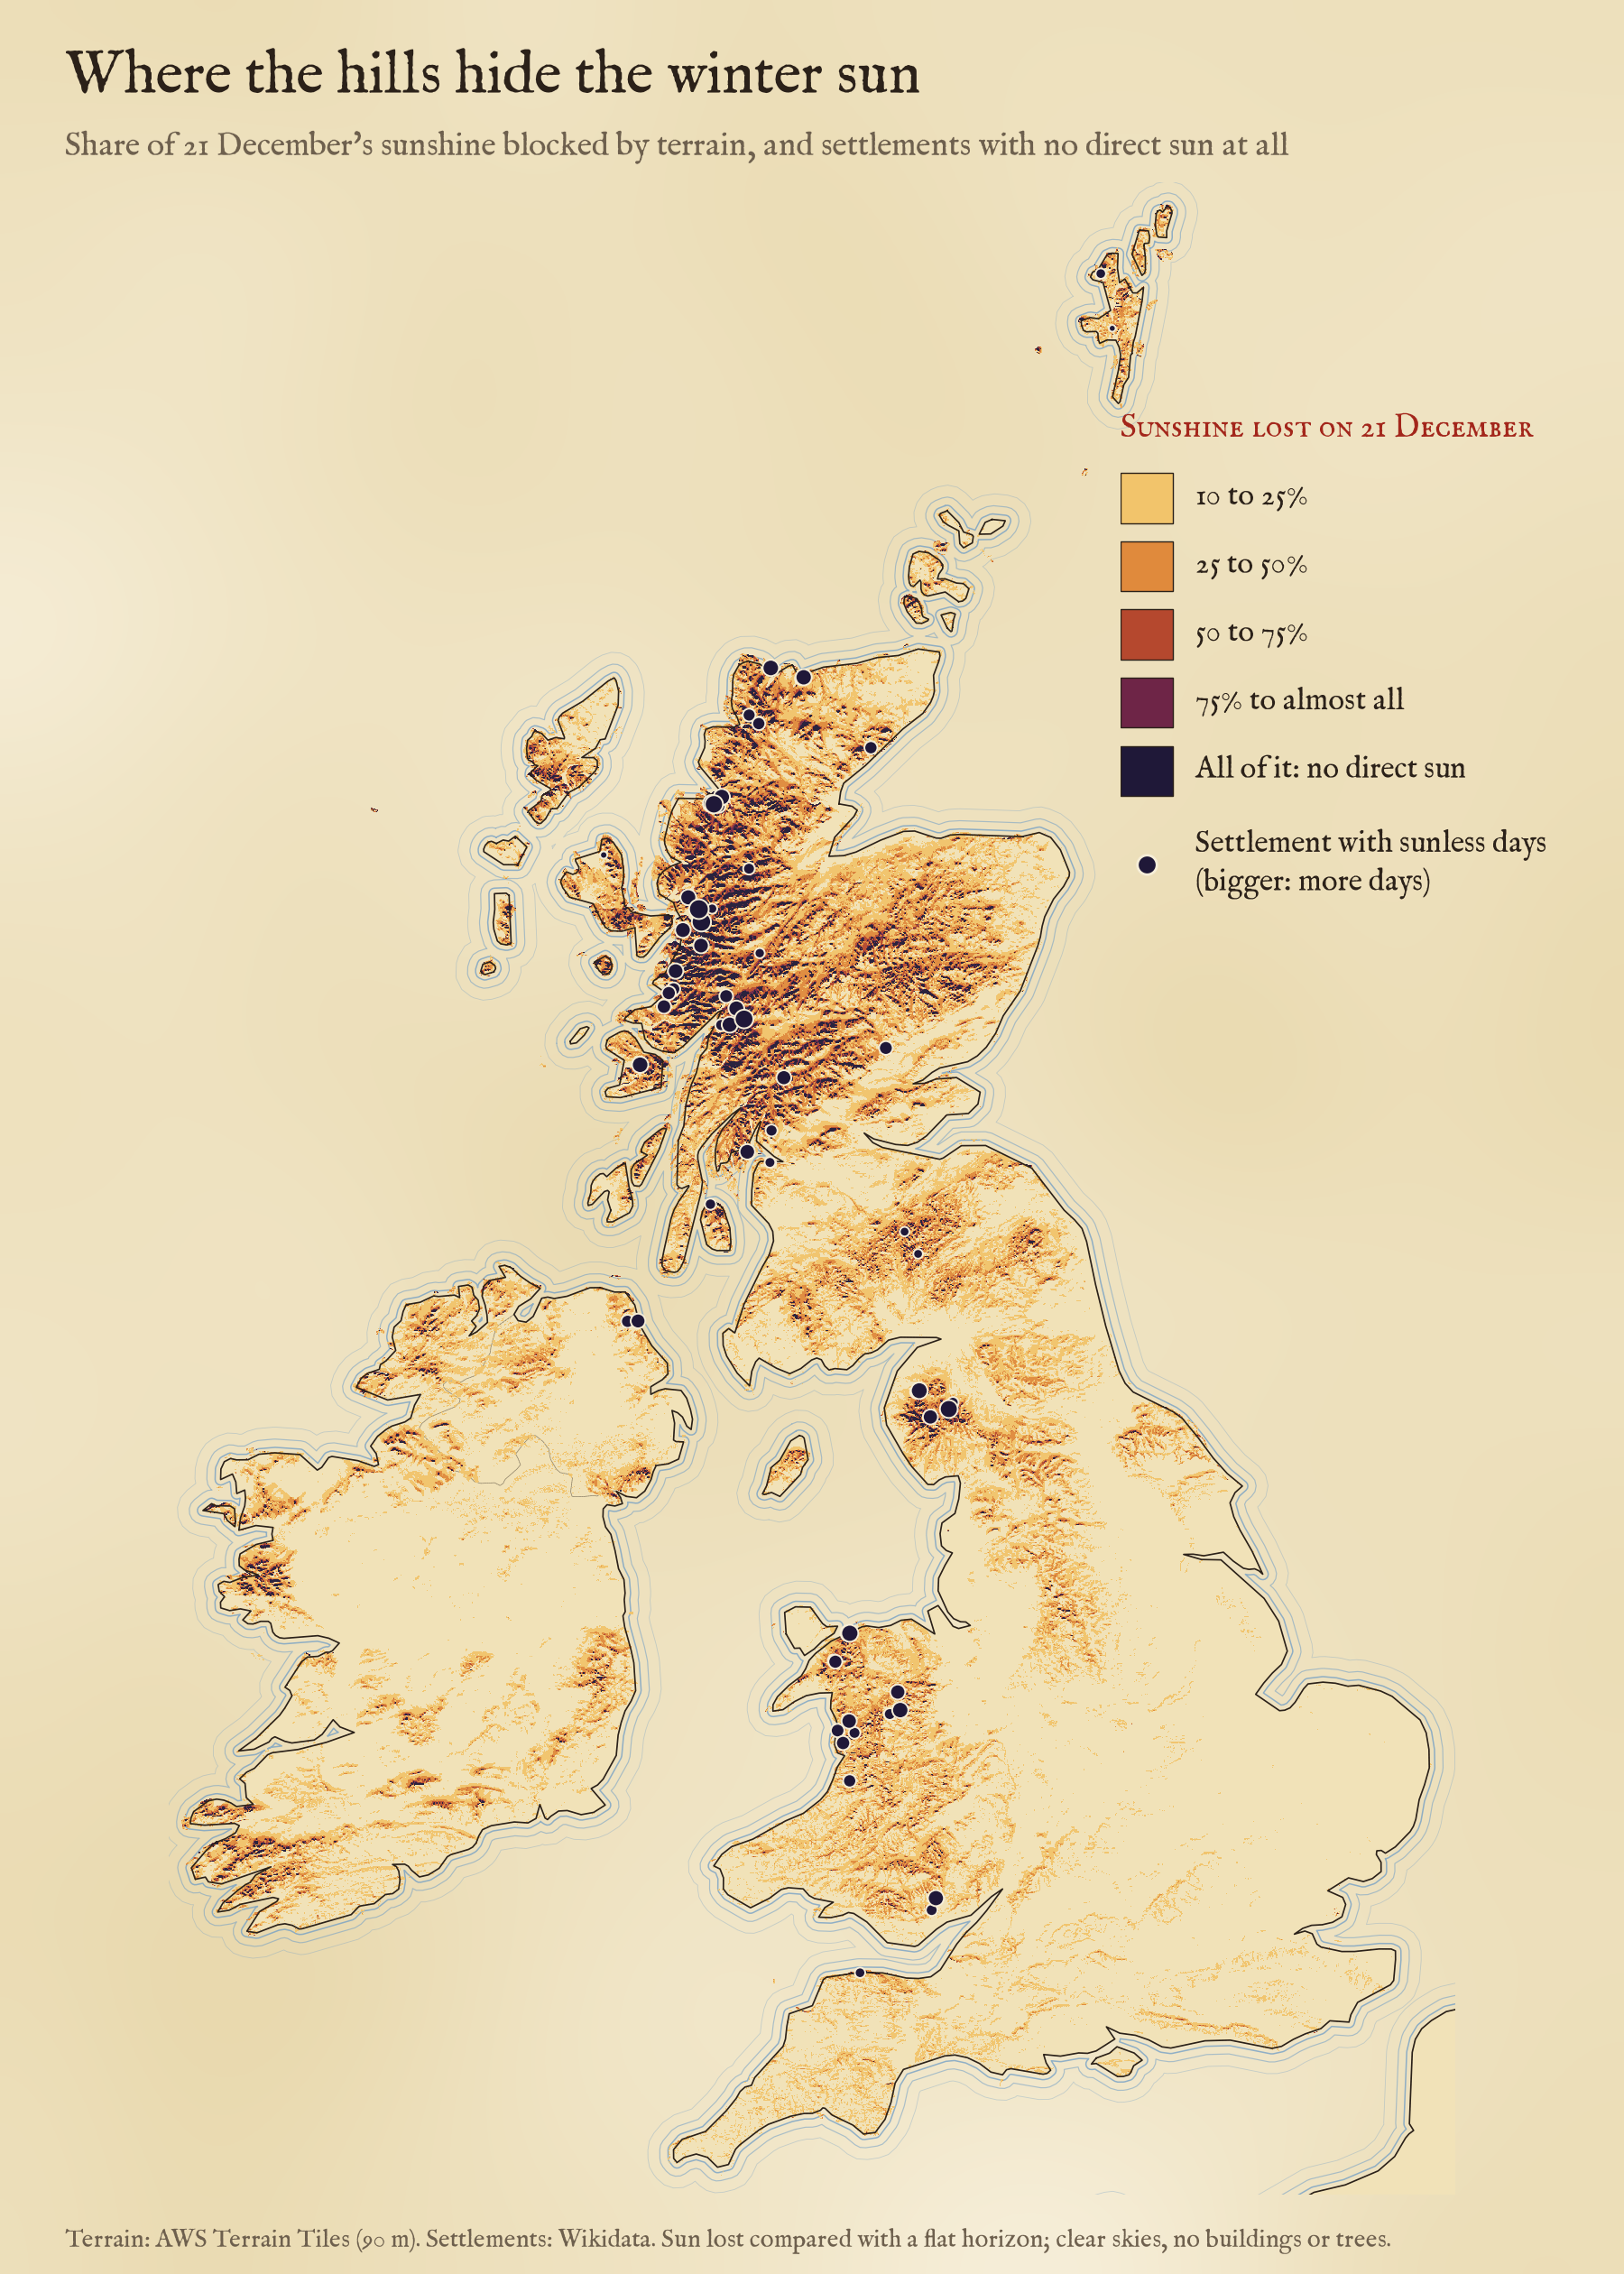
\includegraphics[width=0.84\textwidth]{f_britain.png}
\caption{Share of the sunshine of 21 December blocked by terrain, against a flat horizon, on squares of about 175 m (shown here at the coarser resolution of the page, as the maximum of each 2 by 2 block). Dots: settlements with no direct sun on the solstice, sized by the run of sunless days.}\label{fig:britain}\end{figure}

\subsection{The longest runs without sun}
Table~\ref{tab:top} lists the settlements with the longest runs. They lie in east to west valleys and on north-facing shores under steep southern walls: Kintail and Loch Duich, Loch Leven, Little Loch Broom, the north coast of Sutherland, Skye and Mull in the Highlands and islands; Glencoyne, Borrowdale and the northern fells in the Lake District; the Conwy coast and the Berwyns in Wales. Kinlochleven (population 810) has a horizon 25.6\textdegree{} high due south against a noon sun of 9.9\textdegree{} on the solstice, and no direct sun for 109 days, from about 28 October to 13 February (Figure~\ref{fig:skylines}).

\begin{table}[tbp]\centering\small\caption{The settlements with the longest runs of days without direct sun: ground height (m), horizon due south and noon solar altitude on 21 December (degrees), and the run of sunless days.}\label{tab:top}\begin{tabular}{llrrrrl}\toprule Settlement & County & Height & South horizon & Noon sun & Days & Dates\\\midrule
Camas-luinie & Highland & 19 & 23.8 & 9.4 & 123 & 21 Oct to 20 Feb\\
Morvich & Highland & 59 & 28.7 & 9.4 & 117 & 24 Oct to 17 Feb\\
Kinlochleven & Highland & 14 & 25.6 & 9.9 & 109 & 28 Oct to 13 Feb\\
Camusnagaul & Highland & 27 & 25.9 & 8.8 & 103 & 31 Oct to 10 Feb\\
Seldom Seen & Cumbria & 251 & 20.2 & 12.1 & 99 & 2 Nov to 8 Feb\\
Ardessie & Highland & 32 & 15.5 & 8.8 & 91 & 6 Nov to 4 Feb\\
Pen-y-coed & Clwyd & 99 & 20.2 & 13.4 & 89 & 7 Nov to 3 Feb\\
Routenbeck & Cumbria & 124 & 19.1 & 12.0 & 85 & 9 Nov to 1 Feb\\
Penmaenan & Clwyd & 97 & 22.9 & 13.4 & 83 & 10 Nov to 31 Jan\\
Knock & Argyll and Bute & 263 & 17.8 & 10.2 & 81 & 11 Nov to 30 Jan\\
Allt na h-Airbhe & Highland & 37 & 14.4 & 8.8 & 81 & 11 Nov to 30 Jan\\
Sangobeg & Highland & 34 & 14.3 & 8.1 & 81 & 11 Nov to 30 Jan\\
Cwm Llech & Powys & 282 & 21.6 & 13.8 & 79 & 12 Nov to 29 Jan\\
Coldbackie & Highland & 71 & 16.0 & 8.2 & 79 & 12 Nov to 29 Jan\\
Pantygaseg & Gwent & 339 & 21.2 & 14.9 & 77 & 13 Nov to 28 Jan\\
\bottomrule\end{tabular}\end{table}

\begin{figure}[tbp]\centering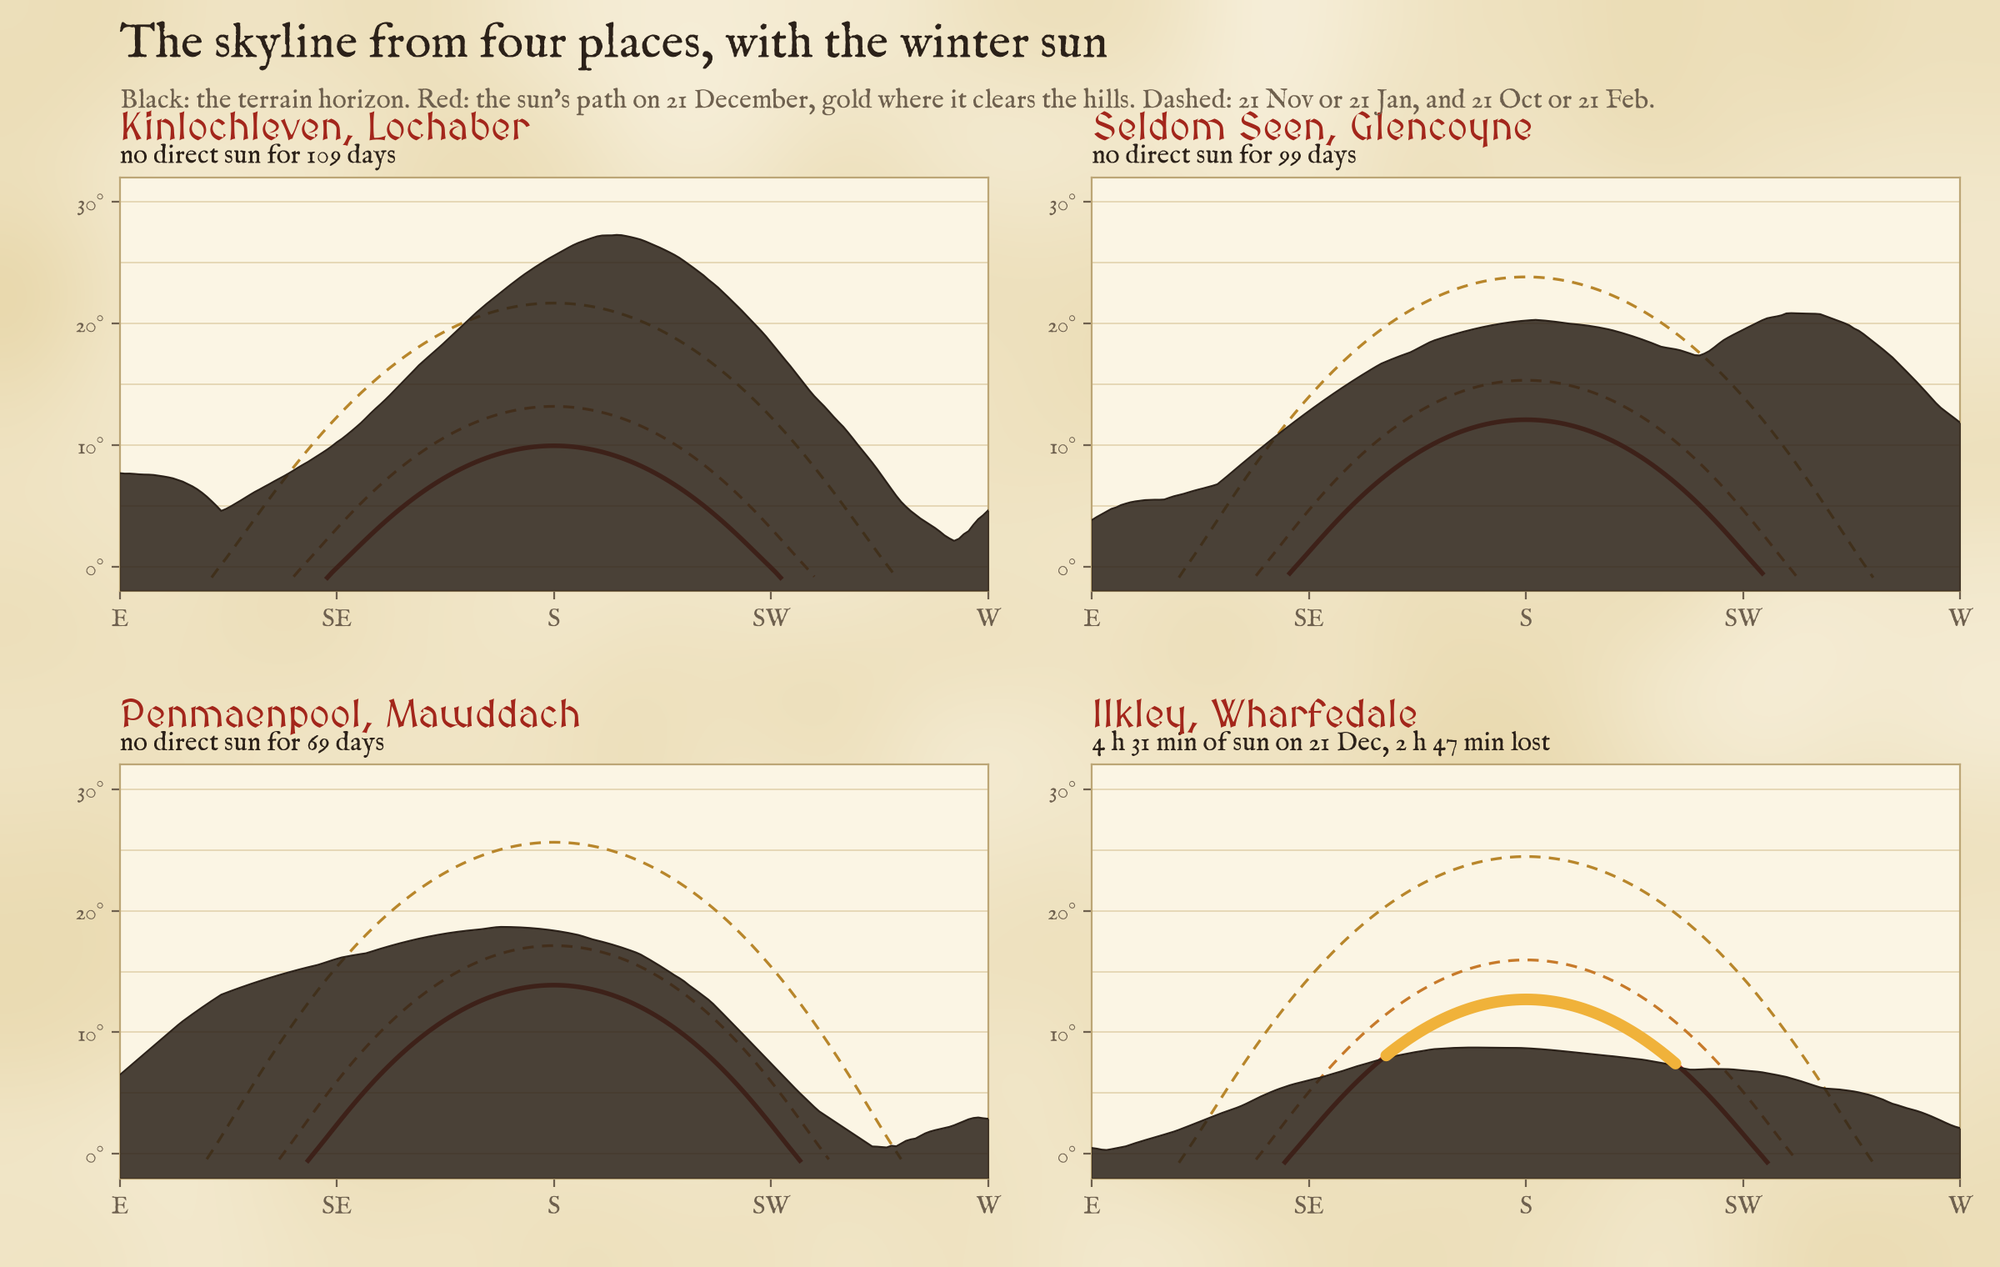
\includegraphics[width=\textwidth]{f_skylines.png}
\caption{Skylines from four settlements (black) with the sun's path on 21 December (red; gold where it clears the terrain) and a month and two months either side (dashed).}\label{fig:skylines}\end{figure}

\begin{figure}[tbp]\centering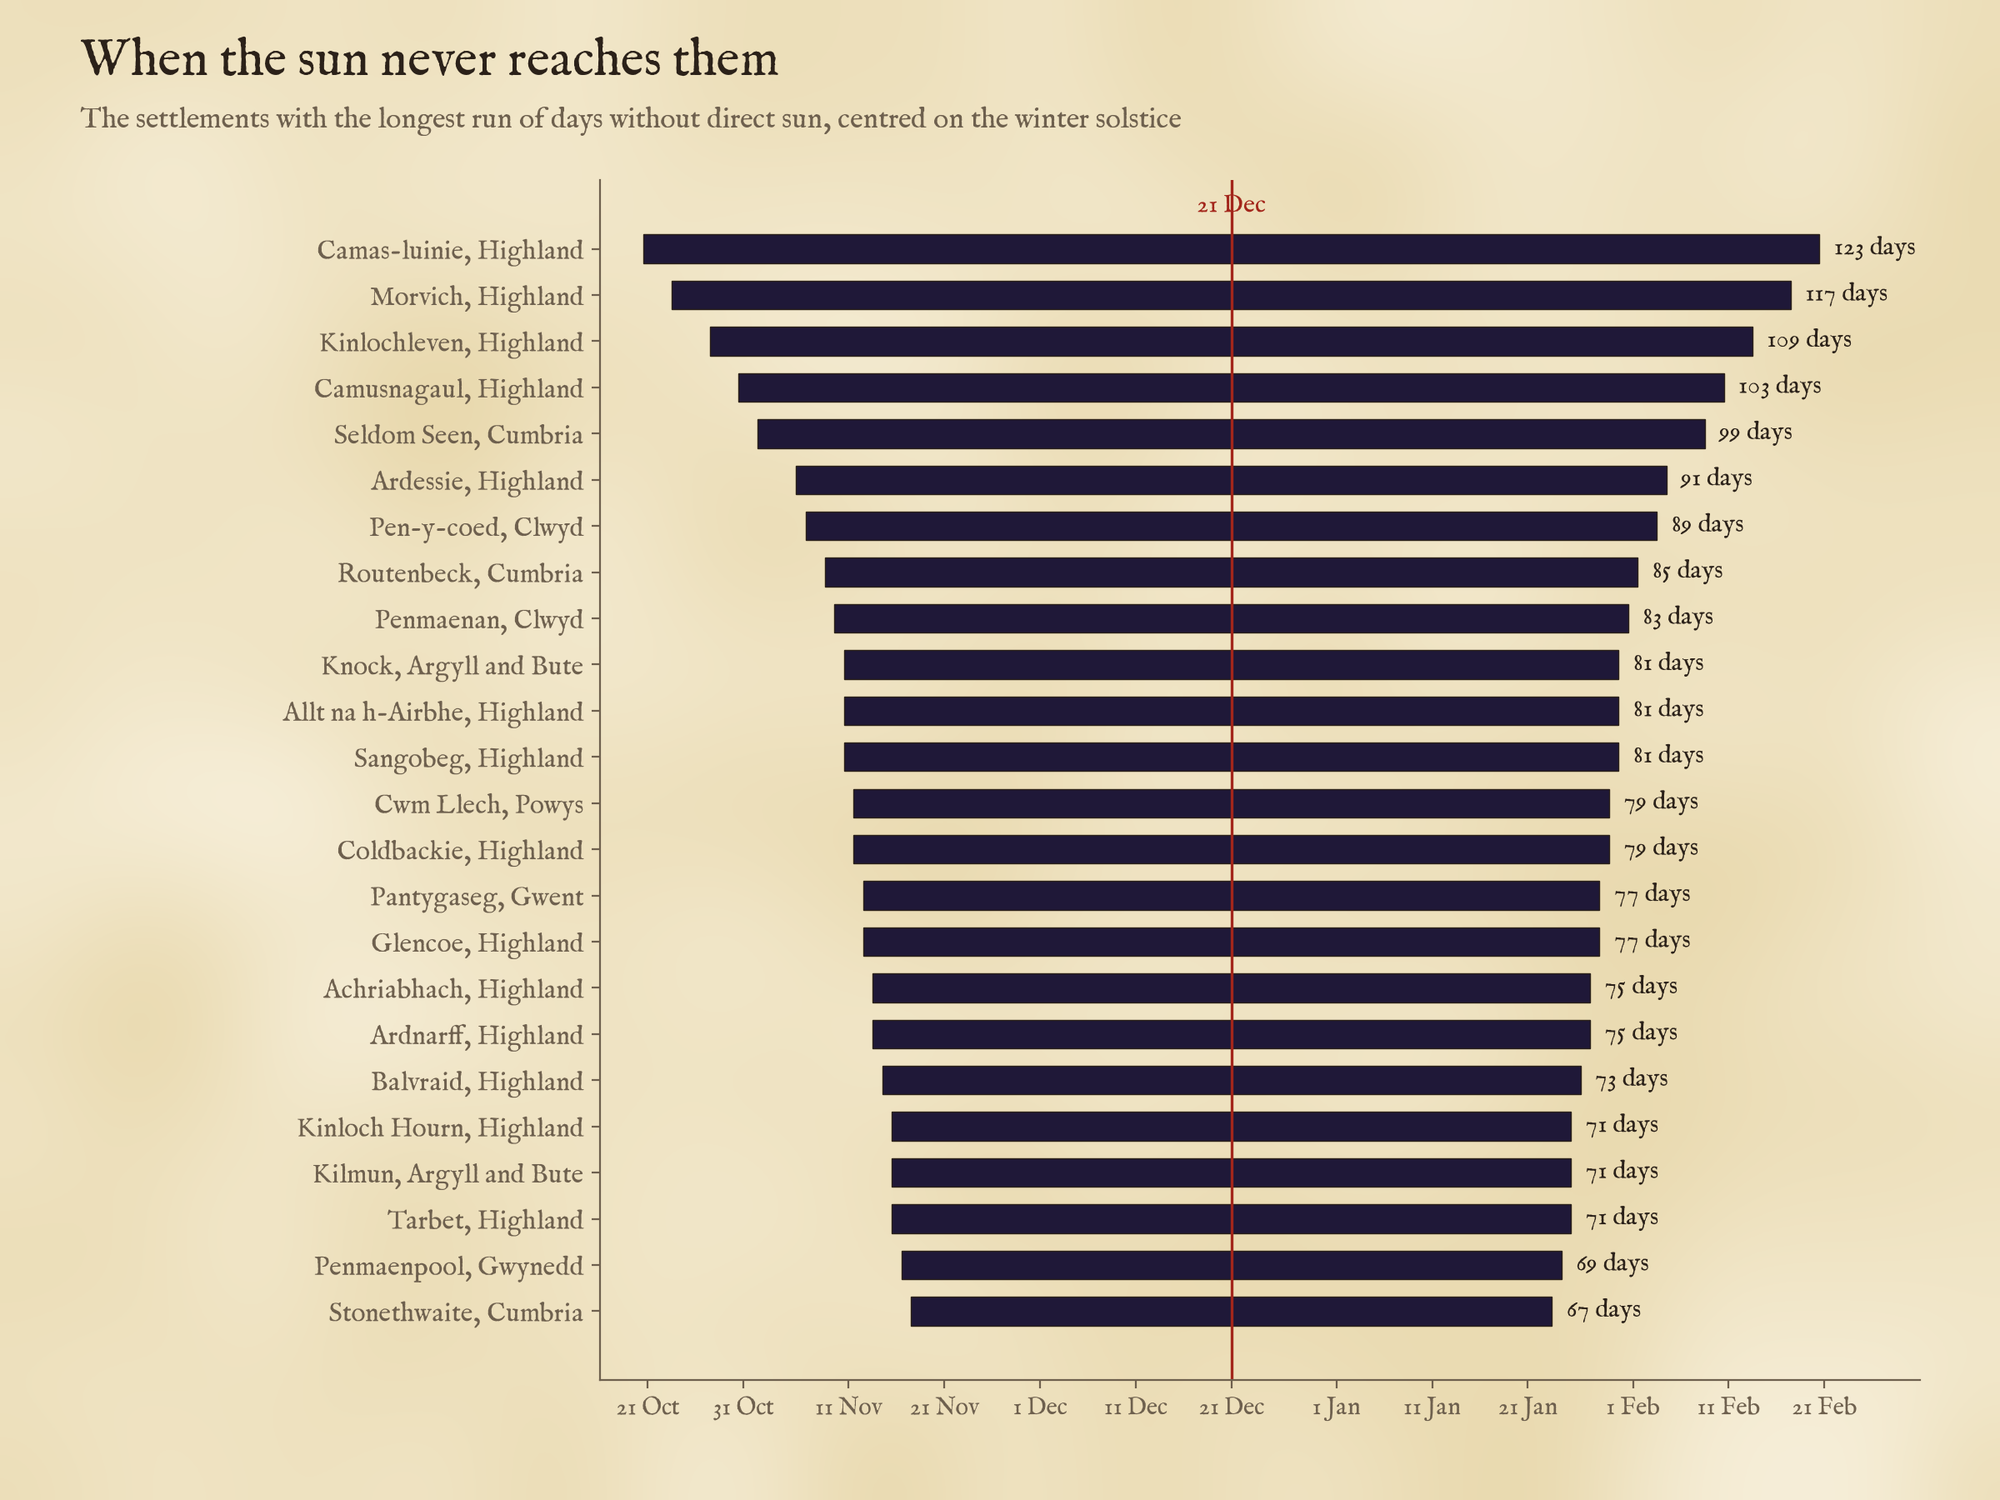
\includegraphics[width=0.92\textwidth]{f_calendar.png}
\caption{The run of days without direct sun for the settlements with the longest runs, centred on the solstice.}\label{fig:calendar}\end{figure}

\subsection{Towns}
Among the 4,589 settlements with a Wikidata population of 2,000 or more, 46 lose two hours or more of solstice sunshine (Figure~\ref{fig:towns}). Penmaenmawr (4,353), under steep hills east of the Penmaen-mawr headland on the Conwy coast, would be the only one to lose all of it, but only at its Wikidata point, west of the town centre; at its OpenStreetMap point in the centre, 0.6 km east, it keeps 1 h 39 min, so it is not counted (Section~\ref{sec:check}). Newburgh in Fife, under the Ochils on the south shore of the Firth of Tay, keeps 47 min. The rest of the list is dominated by the South Wales valleys, and of the 1,663 places of 10,000 or more Ilkley, under Ilkley Moor, loses most (2 h 47 min).

\begin{figure}[tbp]\centering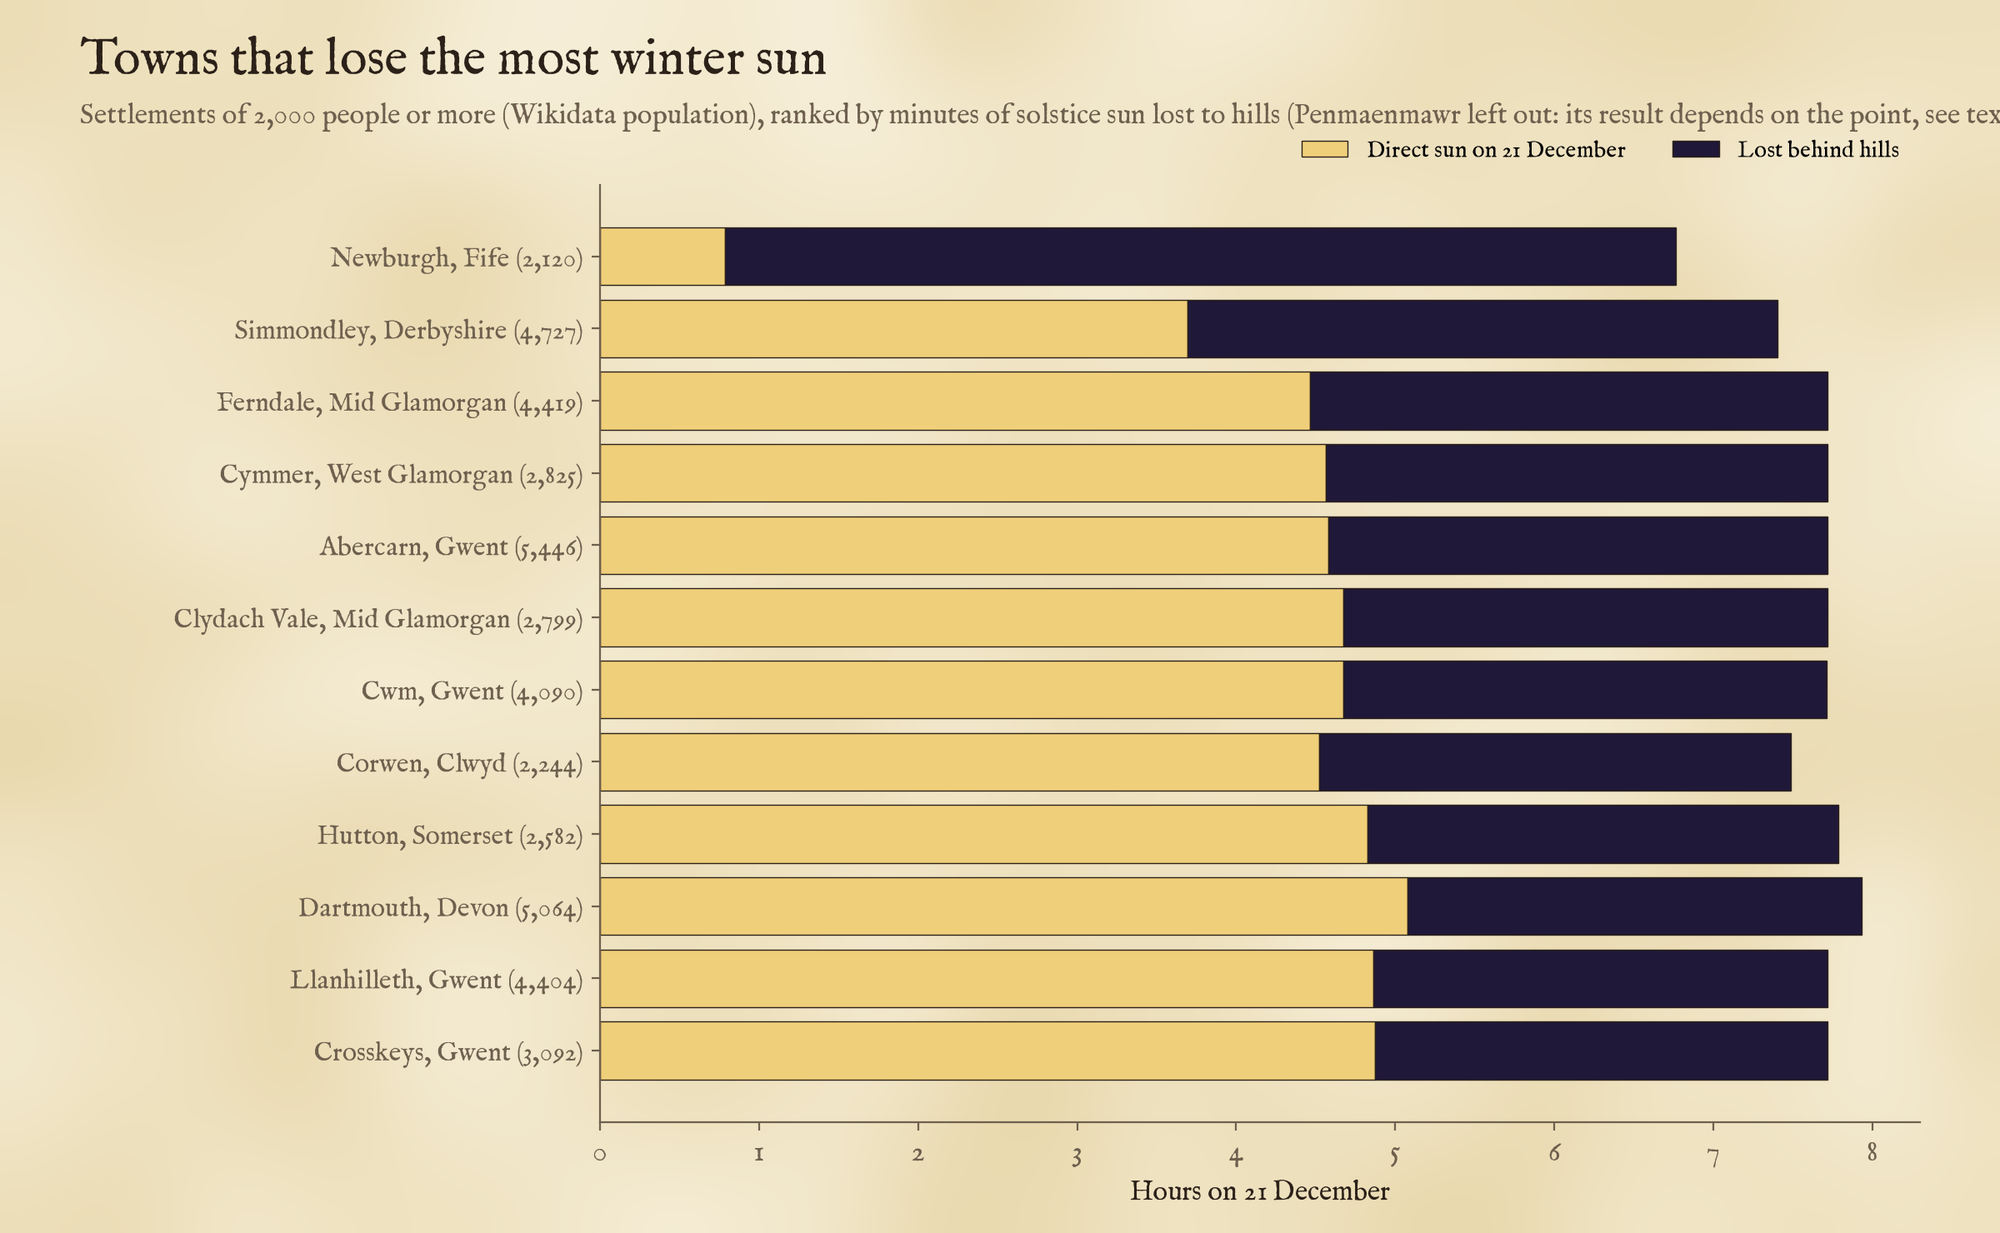
\includegraphics[width=0.92\textwidth]{f_towns.png}
\caption{Settlements of 2,000 people or more losing the most solstice sunshine.}\label{fig:towns}\end{figure}

\subsection{The land}
Over the grid, 4,956 km$^2$ of the United Kingdom (2.04\% of its land) gets no direct sun on 21 December, and 2,451 km$^2$ none for at least 61 days; half or more of the solstice sunshine is lost on 4.6\% (Table~\ref{tab:grid}). Most of this is steep north-facing ground, which shades itself wherever its slope exceeds the sun's altitude. Ireland, for which I had no gazetteer, has 464 km$^2$ without sun on the solstice, 78\% of it in Kerry, Mayo, Donegal and Galway. Figures~\ref{fig:lochaber} and~\ref{fig:lakes} show two of the darkest areas at full resolution.

\begin{table}[tbp]\centering\small\caption{Land in terrain shadow, from the grid: land area, area with no direct sun on 21 December, with none for at least 30 and at least 61 days, and share of land losing half or more of the solstice sunshine (km$^2$). United Kingdom includes coastal cells outside the county outlines.}\label{tab:grid}\begin{tabular}{lrrrrr}\toprule Area & Land & No sun 21 Dec & 30+ days & 61+ days & Half lost\\\midrule
England & 129,364 & 210.3 & 164.3 & 84.2 & 0.5\%\\
Scotland & 76,615 & 4,450.3 & 3,728.5 & 2,252.2 & 12.5\%\\
Wales & 20,486 & 189.3 & 147.0 & 67.3 & 2.8\%\\
Northern Ireland & 14,039 & 35.4 & 27.3 & 12.5 & 0.8\%\\
United Kingdom & 243,330 & 4,956.2 & 4,126.0 & 2,451.2 & 4.6\%\\
Ireland & 69,283 & 464.1 & 383.8 & 221.1 & 1.7\%\\
Isle of Man & 572 & 6.4 & 4.6 & 1.1 & 4.2\%\\
\bottomrule\end{tabular}\end{table}

\begin{figure}[tbp]\centering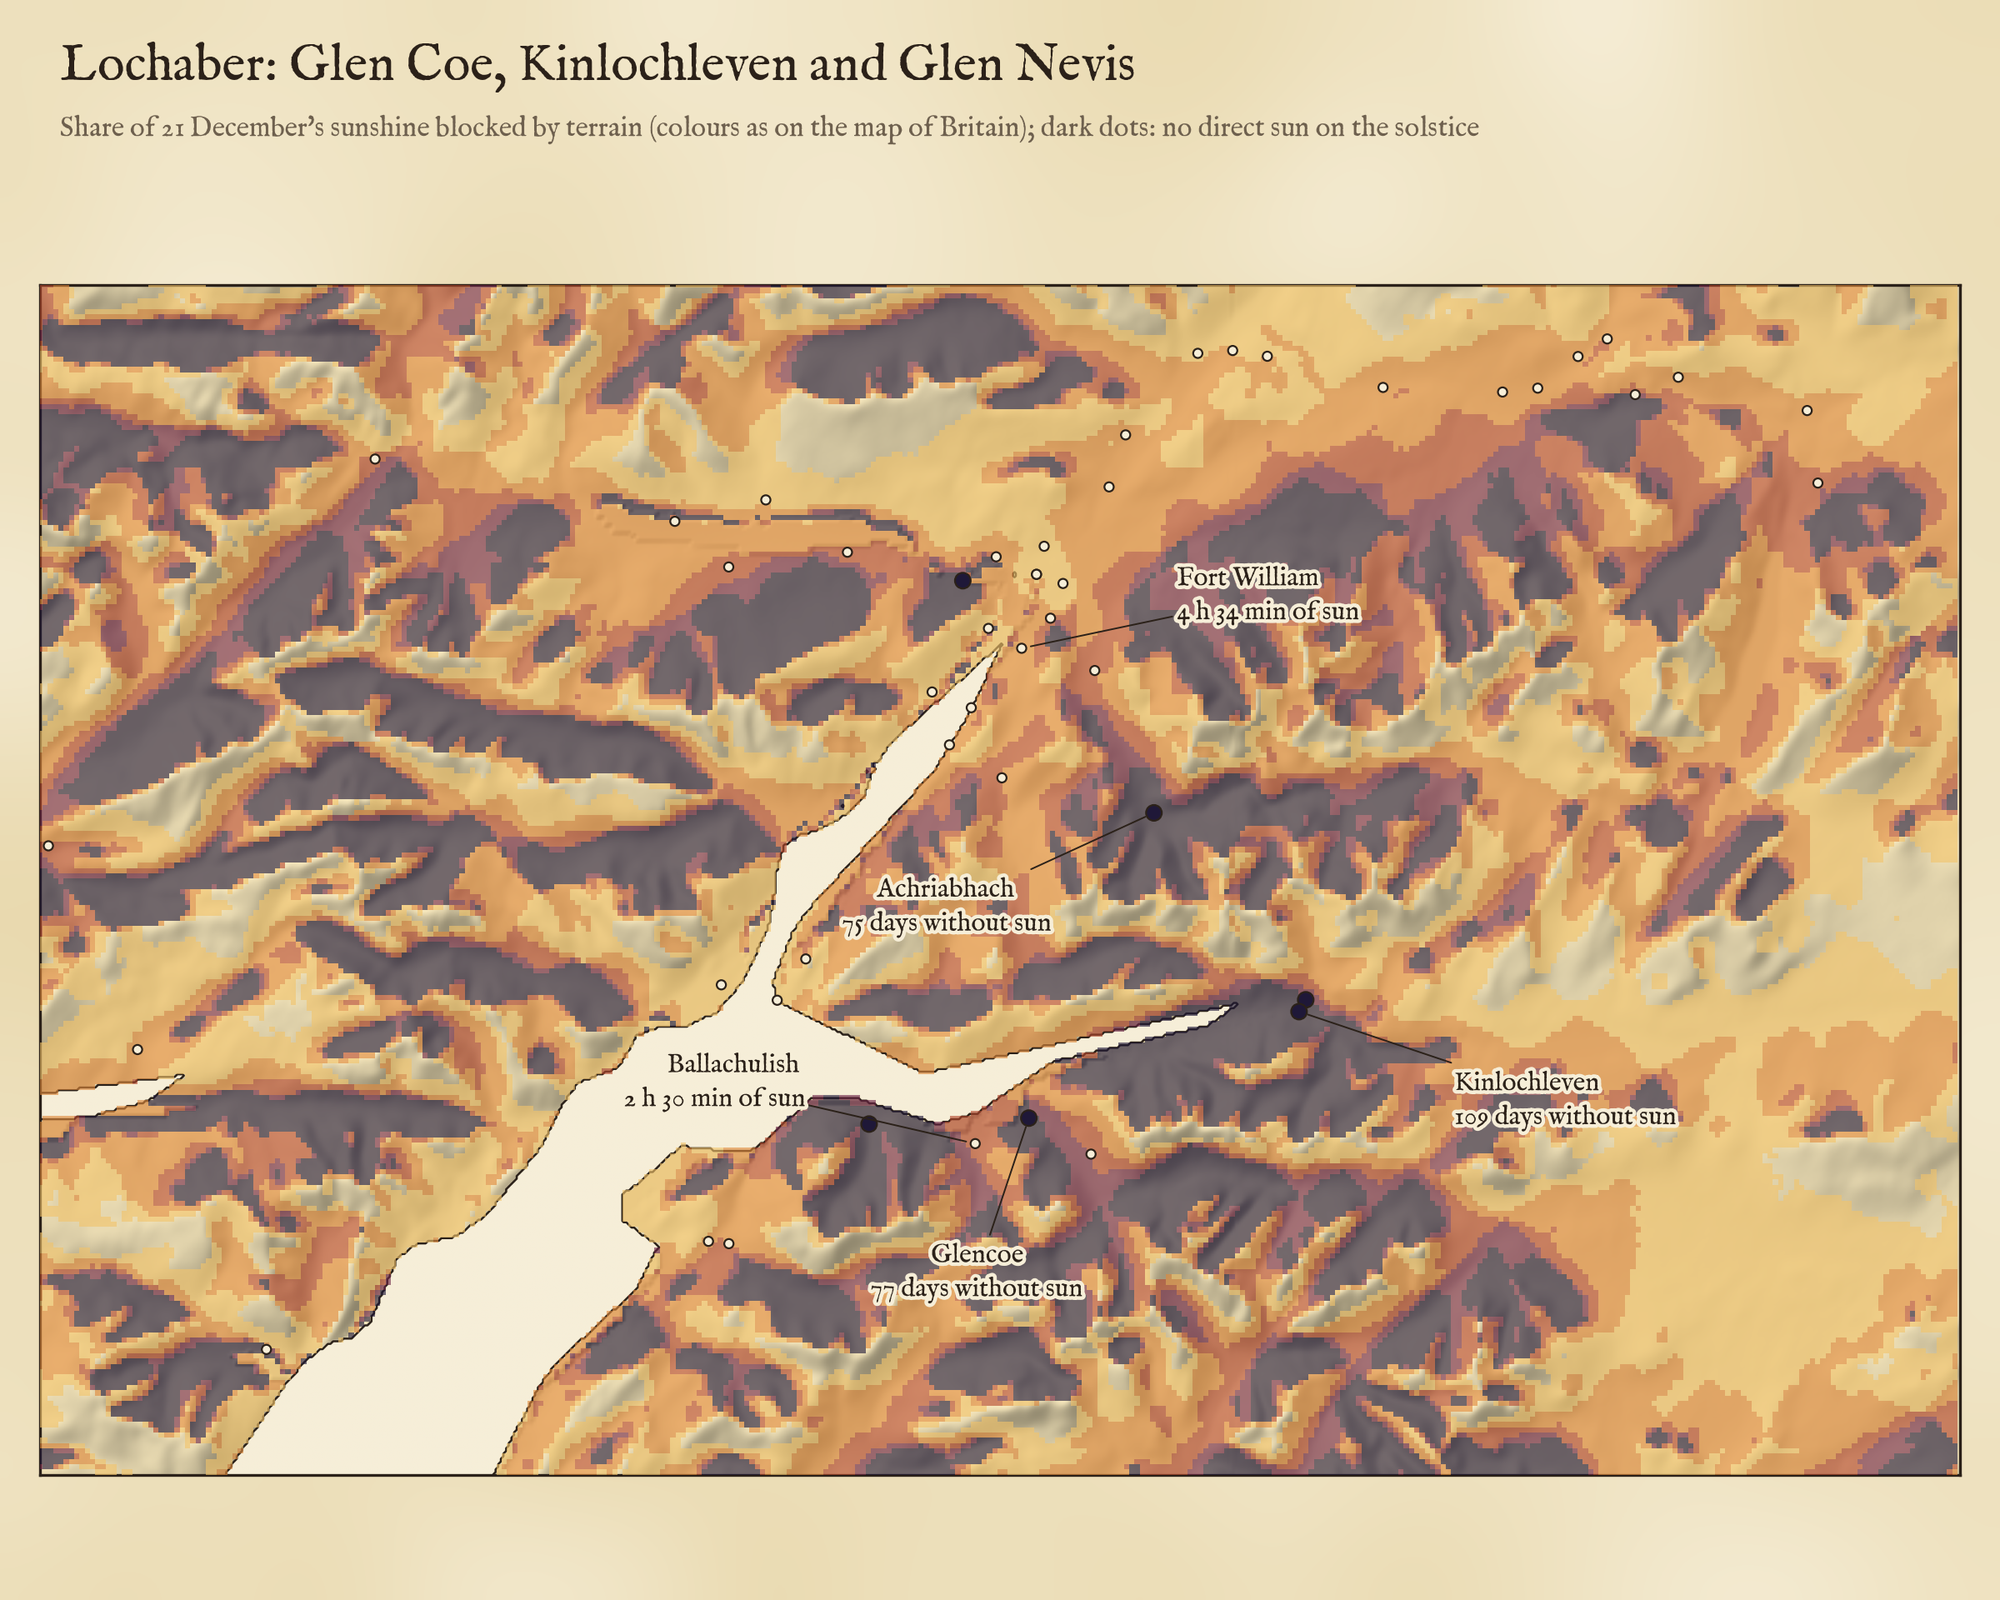
\includegraphics[width=0.92\textwidth]{f_lochaber.png}
\caption{Lochaber: share of the solstice sunshine blocked, over hill shading from the same terrain.}\label{fig:lochaber}\end{figure}
\begin{figure}[tbp]\centering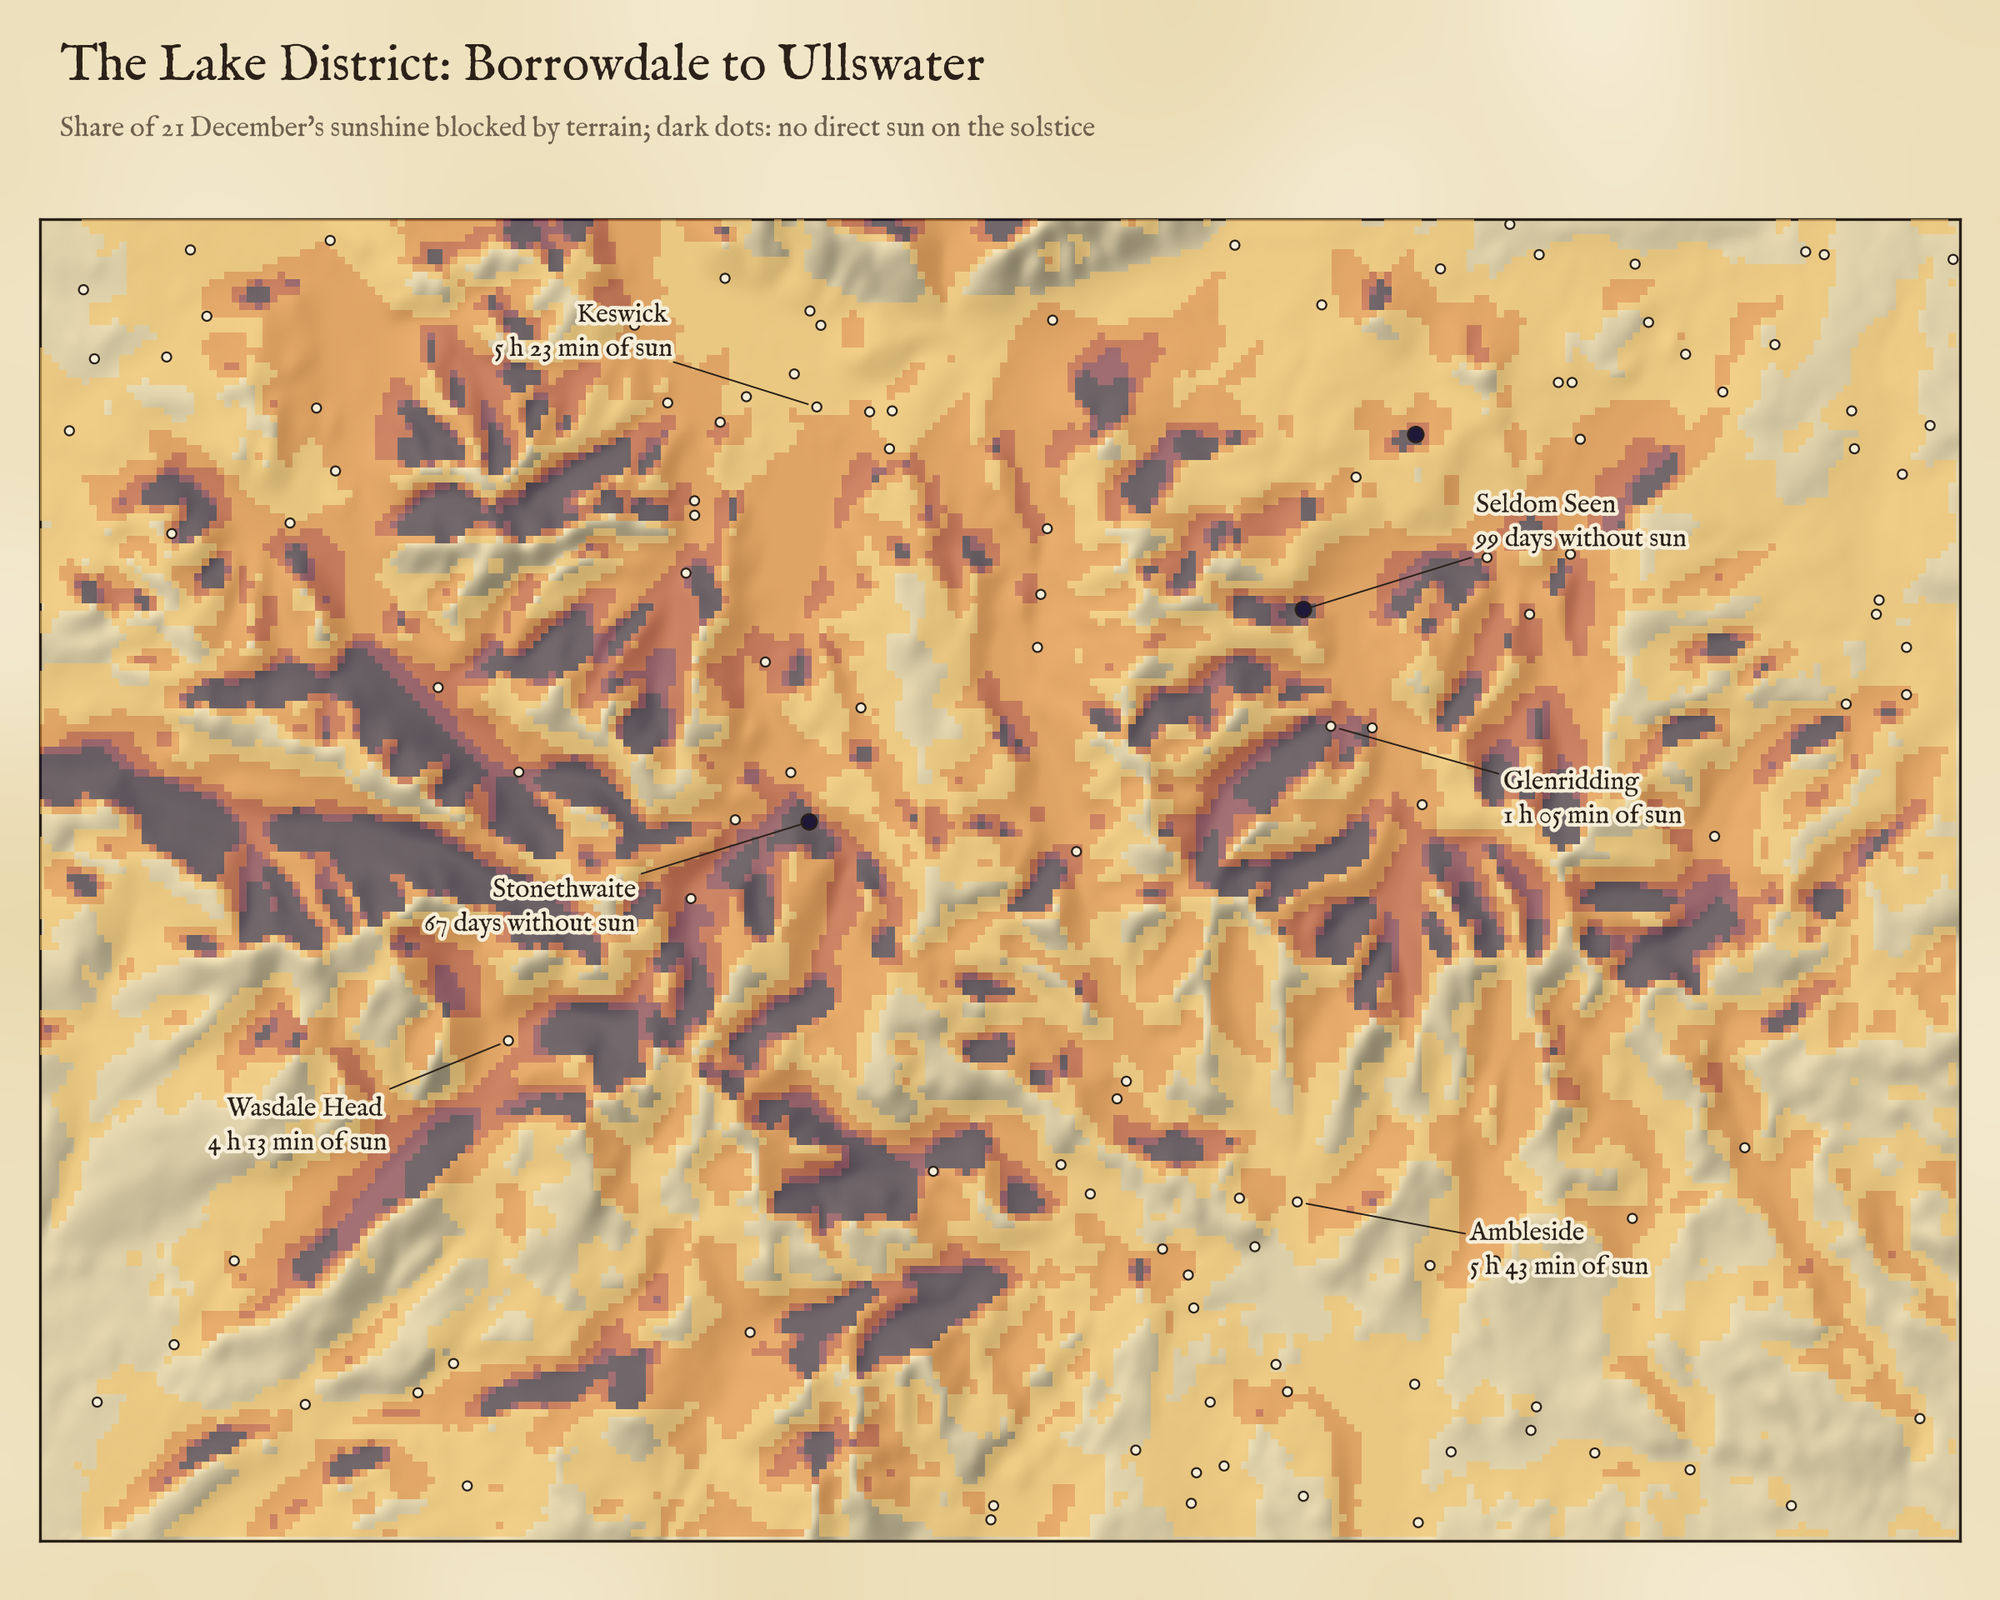
\includegraphics[width=0.92\textwidth]{f_lakes.png}
\caption{The central Lake District, as Figure~\ref{fig:lochaber}.}\label{fig:lakes}\end{figure}

\subsection{Checks}\label{sec:check}
Two checks bear on the sunless settlements. First, separate code recomputed each one from the raw terrain tiles (without despiking), stepping along great circles every 1\textdegree{} of azimuth, with the sun from the NOAA solar position algorithm minute by minute on the real dates of the 2026/27 winter. It finds no direct sun on 21 December at 83 of the 84 points, and runs of sunless days typically 2 days shorter (median), as expected from the coarser sampling near the start and end of a run and the slight asymmetry of the declination about the solstice. Second, the position of the point: for 58 of the 84 an OpenStreetMap place point of the same name lies within about 2 km (OpenFreeMap vector tiles), a median of 0.16 km from the Wikidata point. Moved there, 38 remain without direct sun on the solstice and 20 get some, and these are left out of the count, which is therefore 84 less 20, or 64. They get sun there mostly because the Wikidata point lies a little way up a north-facing slope (Leirinmore, Talisker, Aultbea and Kingairloch among them) or, at Penmaenmawr, at one end of the town. 10 of the 84 Wikidata coordinates carry only two decimals (about 1 km). The per-place results of both checks are in \texttt{data/point\_check.csv}. Even so, any single place should be checked on the ground.

\section{Limitations}\label{sec:limits}
The terrain model is about 90 m across. It smooths narrow gorges and sharp ridges, which lowers horizons close to a point, and SRTM measures the top of the canopy in woodland. There are no buildings: in a town the street, not the hill, often decides whether a window sees the sun. The Wikidata point stands for a whole settlement; villages that climb a hillside, or spread along a valley, may have sunny and sunless parts, and the points themselves vary in how carefully they were placed. Refraction near the horizon changes with the weather, so sunrise and sunset behind distant low ground are uncertain by minutes, and a run of sunless days that ends with the sun just grazing a col is sensitive to small errors in height. Cloud is ignored: these are the hours the sun could shine, not the hours it does. The settlement list is Wikidata's and uneven. Ireland is terrain only.

\section{Conclusion}
Terrain takes a little sunshine from almost every settlement on the shortest day, a great deal from the upland valleys of Scotland, Wales and the Lake District, and all of it from 64 places, some of which go more than three months without direct sun. The skyline of any place, with the sun's path drawn over it, can be explored on the interactive page.

\section*{Data and code availability}
The interactive page is at \url{https://maps.tristanhotham.com/sunless-valleys/}. Derived data (every settlement's sun figures, horizon profiles and the map tiles) and code are at \url{https://github.com/Tristan-Hotham/sunless-valleys} and archived with this paper at https://doi.org/10.5281/zenodo.24055580. Text, figures and derived data are CC BY 4.0 and code MIT. Terrain from the AWS Terrain Tiles (open data, attribution as listed by Tilezen); settlements from Wikidata (CC0); place points for the check from OpenStreetMap via OpenFreeMap (ODbL; the OSM coordinates in \texttt{point\_check.csv} are under the ODbL); boundaries from Natural Earth (public domain) and ONS (Open Government Licence v3.0).

\section*{AI statement}
I wrote the text, with drafting and editing assistance from Claude (Anthropic), which also helped prepare the analysis code. I reviewed and checked all text and results.

\begin{thebibliography}{10}
\bibitem[Bennett(1982)]{bennett1982} Bennett, G. G. (1982) The calculation of astronomical refraction in marine navigation. \textit{Journal of Navigation} 35(2), 255 to 259.
\bibitem[blue News(n.d.)]{bluewin} blue News (n.d.) Four months without sun: how do these people manage? \url{https://www.bluewin.ch/en/entertainment/four-months-without-sun-how-do-these-people-manage-2514156.html} (accessed 2026).
\bibitem[Cooper(1969)]{cooper1969} Cooper, P. I. (1969) The absorption of radiation in solar stills. \textit{Solar Energy} 12(3), 333 to 346.
\bibitem[Dozier et al.(1981)]{dozier1981} Dozier, J., Bruno, J. and Downey, P. (1981) A faster solution to the horizon problem. \textit{Computers and Geosciences} 7(2), 145 to 151.
\bibitem[Farr et al.(2007)]{farr2007} Farr, T. G. et al. (2007) The Shuttle Radar Topography Mission. \textit{Reviews of Geophysics} 45(2), RG2004.
\bibitem[Hofierka and \v{S}\'uri(2002)]{hofierka2002} Hofierka, J. and \v{S}\'uri, M. (2002) The solar radiation model for Open source GIS: implementation and applications. \textit{Proceedings of the Open Source GIS, GRASS Users Conference 2002}, Trento.
\bibitem[Optics and Photonics News(2013)]{opn2013} Optics and Photonics News (2013) Mirrors convey sunshine to dark valley town. 13 November 2013. \url{https://www.optica-opn.org/home/newsroom/2013/november/mirrors_convey_sunshine_to_dark_valley_town}
\bibitem[Saemundsson(1986)]{saemundsson1986} Saemundsson, T. (1986) Astronomical refraction. \textit{Sky and Telescope} 72, 70.
\bibitem[Visit Rjukan(n.d.)]{rjukan} Visit Rjukan (n.d.) Sunfestival in Rjukan. \url{https://visitrjukan.com/en/p/sunfestival-in-rjukan/} (accessed 2026).
\bibitem[Vrande\v{c}i\'c and Kr\"otzsch(2014)]{wikidata} Vrande\v{c}i\'c, D. and Kr\"otzsch, M. (2014) Wikidata: a free collaborative knowledgebase. \textit{Communications of the ACM} 57(10), 78 to 85.
\end{thebibliography}
\end{document}
